\subsection{Is k-cleared-cells NP-hard?}

We prove that k-cleared-cells is NP-hard by constructing a reduction from the \textit{Subset sum} problem. The reduction consists of two parts: one part which considers $K > 1$ in the given \textit{Subset sum} instance, and one part which considers the special case $K = 1$. The first part is more complex and consists of five phases, whereas the second part is relatively straightforward.

The goal of each part is to prove the following: 

\begin{quote}
Given a \textit{Subset sum} instance $Q = \{q_1, \ldots, q_a\}, K \in \{1\} ,\{2, 3, \ldots \}$, there exists a solution $S = \{s_1, \ldots, s_b \} \subseteq Q, \sum Q = K$ if and only if there exists a trajectory sequence $\phi$ which clears $k$ cells in game $G$ in some instance of \textit{k-cleared-cells}.
\end{quote}

\subsubsection{The initial gameboard}

The initial gameboard $B_0$ in the constructed \textit{k-cleared-cells} instance is pictured in~\autoref{fig:initial}. It consists of two identical structures which will from here on be referred to as ``wells''. From the figure we can deduce that $B$ is a $2 \left( \sum P + K + 1 \right) \times 10$-sized gameboard.

\begin{figure}[H]
    \centering
    \resizebox{0.5\textwidth}{!}{
    \begin{tikzpicture}
        \welldefault{0}{0}
        \welldefault{5}{0}
        \draw[dashed] (0, -1) -- (0, 13);
        \draw[dashed] (10, -1) -- (10, 13);
        \draw[dashed] (-1, 0) -- (11, 0);
        \draw[dashed] (-1, 12) -- (11, 12);
        \draw [decorate,decoration={brace,amplitude=10pt},xshift=-12pt,yshift=0pt]
        (0, 0) -- (0, 10) node [left, black,midway,xshift=-0.5cm]
        {\Huge $2 \left( \sum P + K \right)$ rows};
        \draw [decorate,decoration={brace,amplitude=10pt},xshift=-12pt,yshift=0pt]
        (0, 10) -- (0, 12) node [left, black,midway,xshift=-0.5cm]
        {\Huge 2 rows};
        \draw [decorate,decoration={brace,amplitude=10pt,mirror},xshift=0pt,yshift=-12pt]
        (0, 0) -- (9, 0) node [below,black,midway,yshift=-0.5cm]
        {\Huge $10$ columns};
    \end{tikzpicture}
    }
    \caption{The initial gameboard}
    \label{fig:initial}
\end{figure}

A schematic of the well structure is pictured in~\autoref{fig:wells}. Column 5 of the well is empty, the content in the other columns depends on which section the rows are in. A well is divided into the following three sections:

\begin{itemize}
\item The bottom section consists of rows in the interval $\left[ 1, 2 \left( K+1 \right) \right]$. In this section, column 1 and 2 is checkered, column 3 consists of white cells, and column 4 consists of black cells.

\item The middle section consists of rows in the interval $\left[ 2 \left( K+1 \right) +1, 2 \left( K-1 + \sum P \right) \right]$. In this section, column 1 to 3 is checkered, and column 4 consists of black cells.

\item The top section consists of the rows in the interval $\left[2 \left( K-1 + \sum P \right) +1, 2 \left( K + \sum P \right) \right]$. In this section columns 2 and 3 are empty. Column 1 consists of white cell in the bottom row, and one white cell in the top row. Column 4 consists of two white cells.

\end{itemize}

\begin{figure}[H]
    \centering
    \resizebox{!}{0.3\paperheight}{
    \begin{tikzpicture}
        \welldetailed{0}{0}
        \draw[dashed] (-1, 0) -- (6, 0);
        \draw[dashed] (-1, 14) -- (6, 14);
        \draw[dashed] (-1, 16) -- (6, 16);
        \draw[dashed] (-1, 18) -- (6, 18);
        \draw[dashed] (-1, 6) -- (6, 6);
        \draw[dashed] (5, 0) -- (5, 18);
        \node at (0.5, -0.5) {\large 1};
        \node at (1.5, -0.5) {\large 2};
        \node at (2.5, -0.5) {\large 3};
        \node at (3.5, -0.5) {\large 4};
        \node at (4.5, -0.5) {\large 5};
        \draw [decorate,decoration={brace,amplitude=10pt},xshift=-12pt,yshift=0pt]
        (0, 0) -- (0, 6) node [left,align=right,black,midway,xshift=-1cm]
        {\huge Bottom section \\ \\
         \huge $2 \left( K-1 \right)$ rows};
        \draw [decorate,decoration={brace,amplitude=10pt},xshift=-12pt,yshift=0pt]
        (0, 6) -- (0, 14) node [left, align=right,black,midway,xshift=-1cm]
        {\huge Middle section \\ \\
         \huge $2 \sum P$ rows};
        \draw [decorate,decoration={brace,amplitude=10pt},xshift=-12pt,yshift=0pt]
        (0, 14) -- (0, 16) node [left, align=right,black,midway,xshift=-1cm]
        {\huge Top section};
        \draw (3.5, 0.5) -- (7, 0.5) node [right, black, xshift=1cm] 
        {\huge row 1};
        \draw (3.5, 6.5) -- (7, 6.5) node [right, black, xshift=1cm, yshift=-1.5cm]
        {\huge row $2 \left( K+1 \right)$};
        \draw (3.5, 5.5) -- (7, 5.5) node [right, black, xshift=1cm, yshift=1.5cm]
        {\huge row $2 \left( K+1 \right) +1$};
        \draw (3.5, 13.5) -- (7, 13.5) node [right, black, xshift=1cm]
        {\huge row $2 \left( K-1+ \sum P \right)$};
    \end{tikzpicture}
    }
    \caption{The well structure}
    \label{fig:wells}
\end{figure}

The purpose of the well is to force the placement of blocks in play. One feature of the well structure is that if we were to drop a block with 2 black cells on the right half in column 4-5, the black right half would drop down and instantly clear itself and the two bottommost cells in column 4. The terrain in column 4 would then collapse, making place for a new block to be placed in the same manner.

This feature cannot be utilized in the default well state though, since fixing a block on the top of column 5 would result in a game over. Would the two right white cells in the top section disappear, this feature becomes available. This characteristic of the well is heavily used in the reduction. We therefore define two states of the well. If the well is \textit{closed}, placing a block in column 4-5 yields a game over, if the well is \textit{open} this placement does not yield a game over. The appearance of the top section corresponding to the two well states is pictured in~\autoref{fig:openclosed}. The reason for this will later become apparent.

\begin{figure}[H]
    \centering
    \begin{subfigure}[b]{0.15\linewidth}
        \resizebox{\linewidth}{!}{
            \begin{tikzpicture}
                \topclosed{0}{0}
            \end{tikzpicture}
        }
        \caption{Closed}
    \end{subfigure}
    \hspace{0.02\linewidth}
    \begin{subfigure}[b]{0.15\linewidth}
        \resizebox{\linewidth}{!}{
            \begin{tikzpicture}
                \topopen{0}{0}
            \end{tikzpicture}
        }
        \caption{Open}
    \end{subfigure}
    \caption{Open and closed wells}
    \label{fig:openclosed}
\end{figure}

\subsubsection{Phase 1}
In this phase we transform every $q_i \in Q$ to sequences of game blocks. These sequences will be part of the block states $P_1, \ldots P_n$ in the constructed \textit{k-cleared-cells} instance. The transformation is done by creating a sequence of 1 $\mathbf{H}_{H}$, $q_i$ $\mathbf{H}$ and 1 $\mathbf{H}_H$ blocks (in their initial state) for each give $q_i$.

\begin{figure}[H]
    \centering
    \resizebox{0.4\textwidth}{!}{
    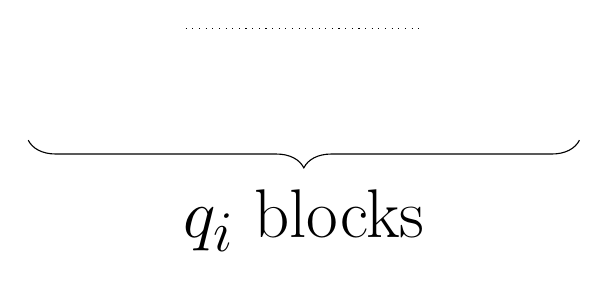
\begin{tikzpicture}
        \startb{0}{0}
        \middleb{3}{0}
        \draw[dotted] (5, 1) -- (8, 1);
        \middleb{8}{0}
        \startb{11}{0}
        \draw [decorate,decoration={brace,amplitude=10pt,mirror},xshift=0pt,yshift=-12pt]
        (3, 0) -- (10, 0) node [below,black,midway,yshift=-0.5cm]
        {\Huge $q_i$ blocks};
    \end{tikzpicture}
    }
    \caption{Transformation of \textit{Subset sum} element $q_i$}
    \label{fig:wells}
\end{figure}
